\chapter[Basic Notions]{Basic notions of radiometric geochronology}
\label{ch:basic-notions}

\section{Isotopes and radioactivity}
\label{sec:isotopes}

Thanks to discoveries by Niels Bohr, Ernest Rutherford, Arnold
Sommerfeld, Joseph Thomson and James Chadwick, we know that rocks and
minerals are made of atoms, atoms are made of a nucleus and an
electron cloud, and the nucleus is made of \emph{nucleons} of which
there are two kinds: protons and neutrons. The total number of
nucleons in the atomic nucleus is called the \emph{mass number}
(A). The number of protons (which equals the number of electrons in a
neutral atom) is called the \emph{atomic number} (Z). The chemical
properties of a nuclide solely depend on the atomic number, which
therefore forms the basis of the Periodic Table of Elements. The
number of neutrons in the atomic nucleus may take on a range of values
for any given element, corresponding to different \emph{isotopes} of
said element. For example, $^{16}_{~8}$O is an isotope of oxygen with
16 nucleons of which 8 are protons (and N = A-Z = 16-8 = 8 are
neutrons). Adding one extra neutron to the nucleus produces a second
oxygen isotope, $^{17}_{~8}$O, with identical chemical properties as
$^{16}_{~8}$O, but slightly different physical properties
(e.g. boiling temperature).  Adding another neutron produces
$^{18}_{~8}$O which, with 8 protons and 10 neutrons, is more than 10\%
heavier than $^{16}_{~8}$O. Due to this mass difference, the
$^{18}_{~8}$O/$^{16}_{~8}$O ratio undergoes \emph{mass fractionation}
by several natural processes, forming the basis of
$^{18}_{~8}$O/$^{16}_{~8}$O palaeothermometry (see the second half of
this course). When we try to add yet another neutron to the atomic
nucleus of oxygen, the nucleus becomes unstable and undergoes
radioactive decay.  Therefore, no $^{19}_{~8}$O exists in nature.

\section{Radioactivity}
\label{sec:radioactivity}

As mentioned before, the Periodic Table of Elements (aka
`Men\-de\-le\-ev's Table') arranges the elements according to the
atomic number and the configuration of the electron cloud. The equally
important \emph{Chart of Nuclides} uses both the number of protons and
neutrons as row and column indices. At low masses, the stable nuclides
are found close to the 1 $\div$ 1 line (N $\approx$ Z), with the
radionuclides found at higher and lower ratios. At higher atomic
numbers, the stable nuclides are found at higher mass numbers,
reflecting the fact that more neutrons are required to keep the
protons together. For example, $^{208}_{~82}$Pb, which is the heaviest
stable nuclide, has 44 more neutrons than protons. The unstable
nuclides (or \emph{radionuclides}), such as $^{209}_{~82}$Pb or
$^{19}_{~8}$O may survive for time periods of femtoseconds to billions
of years depending on the degree of instability, which generally
scales with the `distance' from the curve of stable
nuclides. Radionuclides eventually disintegrate to a stable form by
means of a number of different mechanisms:

\begin{enumerate}
\item{$\alpha$-decay}\\ The atomic nucleus (e.g., $^{238}_{~92}$U,
  $^{235}_{~92}$U, $^{232}_{~90}$Th, $^{147}_{~62}$Sm) loses an
  $\alpha$ particle, i.e. the equivalent of a $^4_2$He nucleus. When
  these nuclei acquire electrons, they turn into Helium atoms, forming
  the basis of the U-Th-He chronometer, which is further discussed in
  Section \ref{sec:U-Th-He}. The recoil energy of the decay is divided
  between the $\alpha$ particle and the parent nucleus, which
  eventually relaxes into its ground state by emitting
  $\gamma$-radiation, i.e. photons with a wavelength of 10$^{-12}$m or
  less.  In addition to the aforementioned U-Th-He method,
  $\alpha$-decay is central to the $^{147}$Sm-$^{143}$Nd (Section
  \ref{sec:Rb-Sr}), $^{235}$U-$^{207}$Pb, $^{238}$U-$^{206}$Pb and
  $^{232}$Th-$^{208}$Pb methods (Section \ref{sec:U-Pb}).

\item{$\beta$-decay}\\ Comprises negatron ($\beta^-$) and positron
  ($\beta^+$) emission, in which either an electron or a positron is
  emitted from the nucleus, causing a transition of (N,Z)
  $\rightarrow$ (N-1,Z+1) for $\beta^-$ decay and (N,Z) $\rightarrow$
  (N+1,Z-1) for $\beta^+$ decay. For example, the oxygen isotope
  $^{19}_{~8}$O discussed in Section \ref{sec:isotopes} decays to
  $^{19}_{~9}$F by $\beta^-$ emission.  In contrast with $\alpha$
  particles, which are characterized by discrete energy levels,
  $\beta$ particles are characterised by a continuous energy
  spectrum. The difference between the maximum kinetic energy and the
  actual kinetic energy of any given emitted electron or positron is
  carried by a neutrino (for $\beta^+$ decay) or an anti-neutrino (for
  $\beta^-$ decay). Just like $\alpha$ decay, $\beta$ decay is also
  accompanied by $\gamma$-radiation, arising from two sources: (a)
  relaxation into the ground state of the excited parent nucleus and
  (b) spontaneous annihilation of the unstable positron in $\beta^+$
  decay. $\beta^-$ decay is important for the $^{40}$K-$^{40}$Ca,
  $^{87}$Rb-$^{87}$Sr (Section \ref{sec:Rb-Sr}) and $^{14}$C-$^{14}$N
  (Section \ref{sec:14C}) clocks. It also occurs as part of the
  $^{235}$U-$^{207}$Pb, $^{238}$U-$^{206}$Pb and $^{232}$Th-$^{208}$Pb
  decay series (Sections \ref{sec:U-Pb} and
  \ref{ch:intro2Useries}). $\beta^+$ decay is found in the
  $^{40}$K-$^{40}$Ar system (Section \ref{sec:K-Ar}).

\item{electron capture}\\ This is a special form of decay in which an
  `extra-nuclear' electron (generally from the K-shell) is captured by
  the nucleus. This causes a transformation of (N,Z) $\rightarrow$
  (N+1,Z-1), similar to positron emission, with which it often
  co-exists. The vacant electron position in the K-shell is filled with
  an electron from a higher shell, releasing X-rays ($\sim$
  10$^{-10}$m wavelength), which is the diagnostic signal of electron
  capture. This mechanism occurs in the
  \textsuperscript{40}K-\textsuperscript{40}Ar decay scheme (Section
  \ref{sec:K-Ar}).

\item{nuclear fission}\\ Extremely large nuclei may disintegrate into
  two daughter nuclei of unequal size, releasing large amounts of
  energy ($\sim$ 200 MeV). The two daughter nuclei move in opposite
  directions from the parent location, damaging the crystal lattice of
  the host mineral in their wake. The two daughter nuclides are
  generally radioactive themselves, giving rise to $\beta$-radiation
  before coming to rest as stable isotopes.  $^{238}_{~92}$U is the
  only naturally occurring nuclide that undergoes this type of
  radioactive decay in measurable quantities, and even then it only
  occurs once for every $\sim$2$\times$10$^6$ $\alpha$-decay events.
  Nevertheless, the fission mechanism forms the basis of an important
  geochronological method, in which the damage zones or `fission
  tracks' are counted (Section \ref{sec:fission-tracks}). Nuclear
  fission can also be artificially induced, by neutron irradiation of
  $^{235}$U, e.g.:

\begin{equation}
{}^{235}_{~92}\mathrm{U} + \mathrm{n} \rightarrow
{}^{236}_{~92}\mathrm{U} \rightarrow {}^{90}_{36}\mathrm{Kr} +
{}^{143}_{~56}\mathrm{Ba} + 3\mathrm{n} + \mbox{energy}
\label{eq:235Ufission}
\end{equation}

Note that every neutron on the left hand side of this formula
generates three neutrons on the right hand side. The latter may react
with further $^{235}$U nuclei and generate a chain reaction. This
forms the basis of nuclear reactors, the atom bomb and the `external
detector' method (Section \ref{sec:fission-tracks}).

\end{enumerate}

\ifpdf
\ifuclnotes
\begin{figure}[!ht]
  \centering
  \def\svgwidth{.7\textwidth}
  \input{chart-of-nuclides.pdf_tex}
  \caption{A schematic `\emph{Chart of Nuclides}' \citep[modified
      from][]{allegre2008}.}
  \label{fig:chart-of-nuclides}
\end{figure}
\else % end of uclnotes
\noindent\begin{minipage}[t]{.6\textwidth}
\strut\vspace*{-\baselineskip}\newline
\def\svgwidth{\textwidth}
\input{chart-of-nuclides.pdf_tex}
\end{minipage}
\begin{minipage}[t]{.4\textwidth}
  \captionof{figure}{A schematic `\emph{Chart of Nuclides}' \citep[modified
      from][]{allegre2008}.}
  \label{fig:chart-of-nuclides}
\end{minipage}
\fi % end of pdf
\else
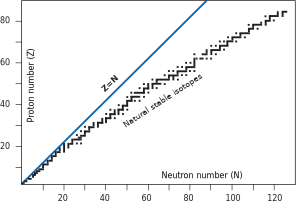
\includegraphics[width=10cm]{../figures/chart-of-nuclides.png}
\captionof{figure}{A schematic `\emph{Chart of Nuclides}' \citep[modified
    from][]{allegre2008}.}
\fi

\section{The age equation}

A characteristic property of radioactive decay is its absolute
independence of external physical and chemical effects. In other
words, it is not affected by changes in pressure, temperature, or the
molecular bonds connecting a radioactive nuclide to neighbouring
atoms. This means that the rate at which a radioactive parent decays
to a radiogenic daughter per unit time, i.e. $dP/dt$ only depends on
$P$, the number of parent atoms present. The \emph{decay constant}
$\lambda$ expresses the likelihood that a radioactive disintegration
takes place in any given time (i.e., $\lambda$ has units of atoms per
atoms per year). This can be expressed mathematically with the
following differential equation:

\begin{equation}
\frac{dP}{dt} = -\lambda P
\label{eq:dPdt}
\end{equation}

Integrating this equation over time yields:

\begin{equation}
P = P_\circ e^{-\lambda t}
\label{eq:P}
\end{equation}

where $P_\circ$ is the number of parent atoms present at time
$t=0$.  Since this number is generally unknown (one exception is
$^{14}$C, see Section \ref{sec:14C}), Equation \ref{eq:P} generally
cannot be used in this form. We can, however, measure the
\emph{present} number of parent and daughter nuclides in the
sample. Rewriting Equation \ref{eq:P}:

\begin{equation}
P_\circ = P e^{\lambda t}
\label{eq:P0}
\end{equation}

and bearing in mind that $P_\circ = P + D$, we obtain:

\begin{equation}
D = P (e^{\lambda t}- 1)
\label{eq:D}
\end{equation}

This equation forms the foundation of most geochronological
methods. It can be rewritten explicitly as a function of time:

\begin{equation}
t = \frac{1}{\lambda} \ln\left(\frac{D}{P} + 1\right)
\label{eq:t}
\end{equation}

The degree of instability of a radioactive nuclide can be expressed by
$\lambda$ or by the \emph{half life} $t_{1/2}$, which is the time
required for half of the parent nuclides to decay. This follows
directly from Equation \ref{eq:P}:

\begin{equation}
\frac{P_\circ}{2} = P_\circ e^{-\lambda t_{1/2}} 
\Rightarrow t_{1/2} = \frac{\ln(2)}{\lambda}
\label{eq:T12}
\end{equation}

As a rule of thumb, the detection limit of a radiometric
geo\-chro\-no\-me\-ter is reached after about 10 half lives. Thus,
$^{14}$C goes back $\sim$50,000 years, $^{10}$Be 10 million and
$^{40}$K 10 billion years.

\section{Decay series}
\label{sec:decay-series}

Sometimes the radiogenic daughter ($D_1$) of a radioactive parent is
radioactive as well, decaying to a daughter of its own ($D_2$), which
may be radioactive again etc., until a stable daughter ($D_*$) is
reached. Considering the simplest case of one intermediate daughter:

\begin{equation}
P \xrightarrow[]{\lambda_P} D_1 \xrightarrow[]{\lambda_1} D_*
\label{eq:series}
\end{equation}

The increase (or decrease) of the number of atoms per unit time for
each of the nuclides is given by:

\begin{align}
\mbox{for~} P &: dP/dt = -\lambda_P P \label{eq:P1}\\
\mbox{for~} D_1 &: dD_1/dt = \lambda_P P - \lambda_1 D_1 \label{eq:D1}\\
\mbox{for~} D_* &: dD_*/dt = \lambda_1 D_1 \label{eq:D*}
\end{align}

The number of parent atoms $P$ can be written as a function of $t$:

\begin{equation}
P = P_\circ e^{-\lambda_P t}
\label{eq:P2}
\end{equation}

Plugging Equation \ref{eq:P2} into \ref{eq:D1} yields

\begin{equation}
dD_1/dt = \lambda_P P_\circ e^{-\lambda_P t} - \lambda_1 D_1
\label{eq:dD1dt}
\end{equation}

Solving this differential equation yields the evolution of $D_1$ with
time. Assuming that $D_1=0$ at $t=0$:

\begin{equation}
D_1 = \frac{\lambda_P}{\lambda_1 - \lambda_P} P_\circ \left[
  e^{-\lambda_P t} - e^{-\lambda_1 t}\right]
\label{eq:ND1}
\end{equation}

If $\lambda_P \ll \lambda_1$ (by a factor of 10 or greater), and $t
\gg 1/\lambda_1$ then $e^{-\lambda_1 t}$ becomes vanishingly small
relative to $e^{-\lambda_P t}$ so that Equation \ref{eq:ND1} can be
simplified:

\begin{equation}
D_1 = \frac{\lambda_P}{\lambda_1 - \lambda_P} P_\circ e^{-\lambda_P t}
\label{eq:ND1b}
\end{equation}

\noindent or, alternatively:

\begin{equation}
D_1 = \frac{\lambda_P}{\lambda_1 - \lambda_P} P
\label{eq:ND1c}
\end{equation}

This means that the ratio of $D_1$ and $P$ remains constant
through time. If $\lambda_P \ll \lambda_1$, then $\lambda_1 -
\lambda_P \approx \lambda_1$, from which it follows that:

\begin{equation}
D_1 = \frac{\lambda_P}{\lambda_1} P
\label{eq:ND1d}
\end{equation}

Rearranging:

\begin{equation}
D_1 \lambda_1 = P \lambda_P
\label{eq:ND1L1}
\end{equation}

or, equivalently:

\begin{equation}
\frac{P}{D_1} = \frac{t_{1/2}(P)}{t_{1/2}(D_1)}
\label{eq:NPND1}
\end{equation}

This is the \emph{secular equilibrium} in which the number of atoms of
both radioactive members is proportional to their respective half
lives. In the geochronological isotope systems $^{235}$U/$^{207}$Pb,
$^{238}$U/$^{206}$Pb and $^{232}$Th/$^{207}$Pb, the lead isotopes are
the end points of a long decay series comprised of several $\alpha$
and $\beta^-$ disintegrations, in which the decay constants of the
parent nuclide is orders of magnitude shorter than the other nuclides
in the chain. For a decay series like that, Equation \ref{eq:ND1L1}
can be generalised to:

\begin{equation}
D_n \lambda_n = \cdots  = D_2 \lambda_2 = D_1 \lambda_1 = P \lambda_P
\label{eq:NDnLn}
\end{equation}

This means that the entire series is in equilibrium, so that all
members occur in mutually constant proportions. The number of atoms of
the stable end member $D_*$ is given by:

\begin{equation}
D_* = P_\circ - P - D_1 - D_2 - \cdots - D_n
\label{eq:ND*}
\end{equation}

Using Equation \ref{eq:NDnLn}, this becomes:

\begin{equation}
D_* = P_\circ - P - \frac{P \lambda_P}{\lambda_1} - 
\frac{P \lambda_P}{\lambda_2} - \cdots - \frac{P \lambda_P}{\lambda_n}
\label{eq:ND*2}
\end{equation}

or

\begin{equation}
D_* = P_\circ - P \left( 1 + \frac{\lambda_P}{\lambda_1} - 
\frac{\lambda_P}{\lambda_2} - \cdots - \frac{\lambda_P}{\lambda_n}\right)
\label{eq:ND*3}
\end{equation}

Since each of the ratios $\lambda_P/\lambda_1$, $\lambda_P/\lambda_2$,
etc.  are vanishingly small, we can simplify Equation \ref{eq:ND*3}
as:

\begin{equation}
D_* = P_\circ - P = P \left( e^{\lambda_P t} -1 \right)
\label{eq:ND*4}
\end{equation}

This means that the accumulation of the final Pb isotope of the
aforementioned three decay series is only a function of the decay of
the parent isotope.  All intermediate decay steps are therefore
inconsequential. In rare cases, however, the isotopic equilibrium is
disturbed by a dissolution or recrystallisation event, say. The
intermediate parent/daughter pairs can then be used to date phenomena
occurring over much shorter time scales than those probed by the U-Pb
method (Section \ref{ch:intro2Useries}).

\begin{figure}[!ht]
  \captionsetup{width=11cm}
  \centering
  \ifpdf
  \ifuclnotes
  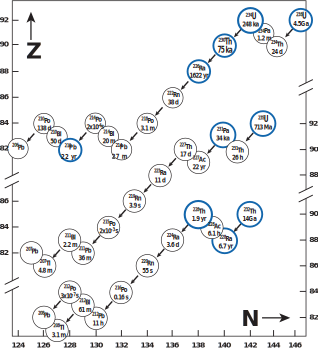
\includegraphics[width=\textwidth]{../figures/U-Th-series.pdf}
  \else
  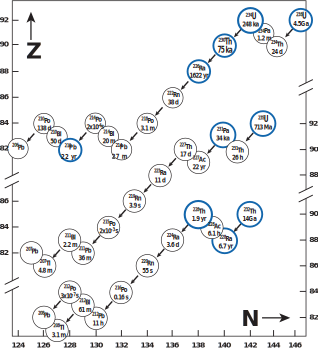
\includegraphics[width=12cm]{../figures/U-Th-series.pdf}
  \fi
  \else
  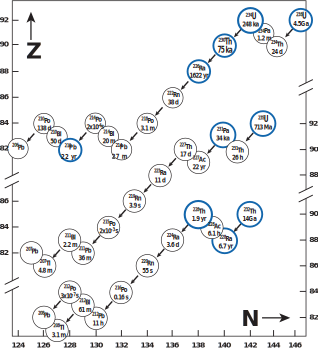
\includegraphics[width=11cm]{../figures/U-Th-series.png}
  \fi
  \caption{The decay series of $^{232}$Th, $^{235}$U and $^{238}$U,
    which form the basis of the U-Th-Pb, U-Th-He and U-Th-series methods
    \citep[modified from][]{allegre2008}.}
  \label{fig:U-Th-series}
\end{figure}
